\documentclass[border=10pt]{standalone}
\usepackage{pgfplots}
\pgfplotsset{compat=1.18}
\begin{document}
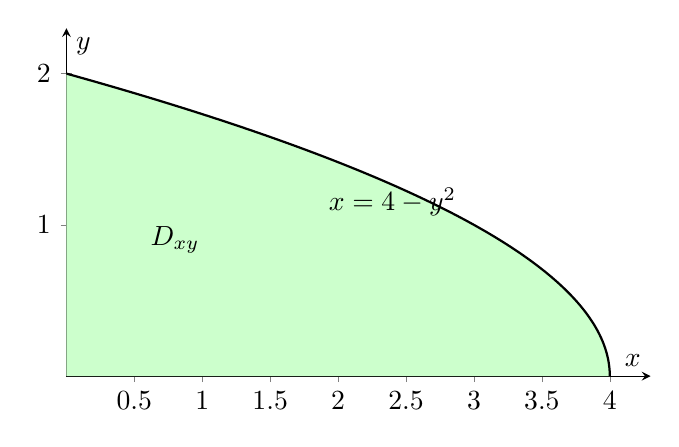
\begin{tikzpicture}
\begin{axis}[
    axis lines=middle,
    xlabel=$x$, ylabel=$y$,
    xmin=0, xmax=4.3, ymin=0, ymax=2.3,
    width=9cm, height=6cm,
    samples=250,
    variable=\t,
    ]
\addplot[fill=green!20, draw=none, domain=0:2] ({4-\t^2}, \t) \closedcycle;
\addplot[domain=0:2, thick, black] ({4-\t^2}, \t);
\node at (axis cs:2.4,1.15) {$x=4-y^2$};
\node at (axis cs:0.8,0.9) {$D_{xy}$};
\end{axis}
\end{tikzpicture}
\end{document}